\section{Introduction: Exponential Growth}
%Before we look at exponential growth, let us recall the familiar concept of \textit{linear growth}.
\begin{example} \label{ex:linear_growth}
	Suppose we have a bank account with 50 CHF in year zero.
	Every year, we deposit 20 CHF.
	This can be visualized in a table.
	%This is visualized in Figure~\ref{fig:linear_exponential_growth} (left).
%	\begin{table}[ht]
%		\centering
%		\begin{tabular}{|l|c|c|c|c|c|c|c|c|c|} \hline
%			year & 0 & 1 & 2 & 3 & 4 & 5 & 6 & 7 & 8 \\ \hline
%			CHF & 50 & 70 & 90 & 110 & 130 & 150 & 170 & 190 & 210 \\ \hline
%		\end{tabular}
%		\label{tab:linear_growth}
%	\end{table}
	\begin{center}
	\begin{tikzpicture}
		\matrix[matrix of math nodes,draw, column sep=1em,row sep=.5mm] (mx) {
			\textrm{year} & 0 & 1 & 2 & 3 & 4 & 5 & 6 & 7 & 8 \\
			\textrm{CHF} & 50 & 70 & 90 & 110 & 130 & 150 & 170 & 190 & 210 \\
		};
		\path[->,shorten >=2pt]
		\foreach \from/\to in {2/3,3/4,4/5,5/6,6/7,7/8,8/9,9/10} {
			([yshift=2mm]mx-1-\from.north) edge[bend left]
			node[above] {$\scriptstyle+1$} ([yshift=2mm]mx-1-\to.north)
			([yshift=-2.5mm]mx-2-\from.south) edge[bend right]
			node[below] {$\scriptstyle+20$} ([yshift=-2.5mm]mx-2-\to.south)
		};
		\foreach \x in {2,...,10}{
			\draw ([xshift=-1em]mx.north west -| mx-1-\x.west) -- ([xshift=-1em]mx.south west -| mx-1-\x.west);
		};
		\draw (mx.west) -- (mx.east);
	\end{tikzpicture}
	\end{center}
	How much money are we going to have in year $x$?
	The answer clearly is (in CHF)
	\begin{equation*}
		20x+50.
	\end{equation*}
	This is an example of \textbf{linear growth}.
\end{example}
\annotation{3}
\begin{exercise} \label{ex:exponential_growth}
	Suppose we have again a bank account with 50 CHF in year zero.
	We will not deposit any money.
	Instead, the bank pays us an interest of 20\% each year.
	For example, if we have 100 CHF on our bank account during a certain year, then we will have 120 CHF in the next year.
	\begin{tasks}
		\task How much money are we going to have in year $x$? Create and fill a table analogously to the one in Example~\ref{ex:linear_growth}.
		How do the tables differ?
		\task Find a function $f\left(x\right)$ that returns the amount of money in year $x$.
		\task Draw the graph of the function $f\left(x\right)$ and compare it to the one in Example~\ref{ex:linear_growth}.
	\end{tasks}
\end{exercise}
\begin{solutions}
\begin{solution*}
	In year zero, we have 50 CHF on our bank account.
	Thus in year one, we will have $60=50\cdot 1.2$ CHF.
	In year two, it will be $72=60\cdot 1.2$ CHF.
	This can also be written as $72=50\cdot 1.2^2$ CHF.
	Following this scheme, we arrive at the solution given below.
	\begin{enumerate}[a)]
		\item The table is given by
%		\begin{tabular}{|l|c|c|c|c|c|c|c|c|c|} \hline
%			year & 0 & 1 & 2 & 3 & 4 & 5 & 6 & 7 & 8 \\ \hline
%			CHF & 50 & 60 & 72 & 86.4 & 103.68 & 124.416 & 149.2992 & 179.15904 & 214.990848 \\ \hline
%		\end{tabular}\\
		\begin{center}
		\begin{tikzpicture}
			\matrix[matrix of math nodes,draw, column sep=1em,row sep=.5mm] (mx) {
				\textrm{year} & 0 & 1 & 2 & 3 & 4 & 5 & 6 & 7 & 8 \\
				\textrm{CHF} & 50 & 60 & 72 & 86.4 & 103.68 & 124.416 & 149.2992 & 179.15904 & 214.990848 \\
			};
			\path[->,shorten >=1pt]
			\foreach \from/\to in {2/3,3/4,4/5,5/6,6/7,7/8,8/9,9/10} {
				([yshift=2mm]mx-1-\from.north) edge[bend left]
				node[above] {$\scriptstyle+1$} ([yshift=2mm]mx-1-\to.north)
				([yshift=-2.5mm]mx-2-\from.south) edge[bend right]
				node[below] {$\scriptstyle\cdot 1.2$} ([yshift=-2.5mm]mx-2-\to.south)
			};
			\foreach \x in {2,...,10}{
				\draw ([xshift=-\x-15]mx.north west -| mx-1-\x.west) -- ([xshift=-\x-15]mx.south west -| mx-1-\x.west);
			};
			\draw (mx.west) -- (mx.east);
		\end{tikzpicture}
		\end{center}
		Note the difference: This time, the function values change by a constant factor!
		\item The function is given by $f\left(x\right)=50\cdot 1.2^x$ CHF.
		\item The graph of $f\left(x\right)$ is given below.
	\end{enumerate}
	\begin{center}
		\includegraphics[width=0.45\textwidth]{images/linear_growth}\hfill
		\includegraphics[width=0.45\textwidth]{images/quadratic_growth}
	\end{center}
\end{solution*}
\end{solutions}
\if\hide1\vspace*{8cm}\fi
\annotation{15}
\begin{tcolorbox}
	We say that a function $f\left(x\right)$ grows \ldots
	\begin{itemize}
		\item[] \ldots\ \textbf{linearly}, if $f\left(x\right)=ax+b$ for some $a>0$, and \ldots
		\item[] \ldots\ \textbf{exponentially}, if $f\left(x\right)=a\cdot b^x$ for some $a>0$ and $b>1$.
	\end{itemize}
\end{tcolorbox}
\begin{example}
	The function in Exercise~\ref{ex:exponential_growth} grows exponentially with $a=50$ CHF and $b=1.2$.
\end{example}
\begin{figure}[ht]
	\centering
	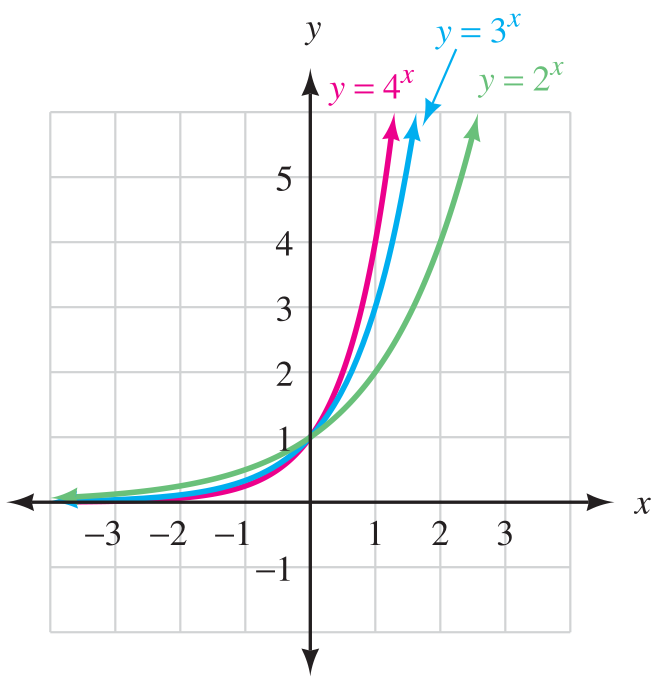
\includegraphics[width=0.40\textwidth]{images/exponentalb}
	\caption{Graph of exponentially growing functions with $a=1$.}
	\label{fig:differentb}
\end{figure}
\annotation{20}
\begin{exercise} \label{ex:first_exponential_equation}
	This time, we have only 20 CHF on our bank account at year zero.
	The bank still pays in interest of 20\% at the end of each year.
	How many years will it take until we have more than 500 CHF on our bank account?
\end{exercise}
\begin{solutions}
\begin{solution*}
	In year $x$, we have $f\left(x\right)=80\cdot 1.2^x$ CHF on our bank account.
	Consequently, we have $f\left(10\right)=495.34$ CHF and $f\left(11\right)=594.41$ CHF (both rounded to two digits).
	Hence it takes 11 years.
\end{solution*}
\end{solutions}
\if\hide1\vspace*{8cm}\fi
\annotation{25}
We have just solved our first \textbf{exponential equation}, i.e. an equation where $x$ occurs in the exponent.
To efficiently solve these equations, we need the inverse function of $b^x$.
Such an inverse function is called \textbf{logarithm}.
\begin{tcolorbox}
	Many quantities in nature grow or decay exponentially.
	\begin{itemize}
		\item Growth of bacteria populations
		\item Radioactive decay
		\item Number of infections during Corona
		\item Human senses (Weber--Fechner law)
		\item \ldots
	\end{itemize}
\end{tcolorbox}
\begin{example}
	Tones that we perceive as rising in equal steps actually grow by a constant factor in terms of frequency.
	For example rising by an octave means doubling the frequency.
	\begin{flushright}
	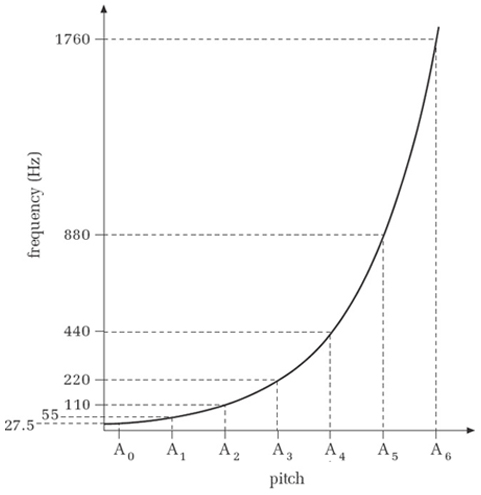
\includegraphics[width=0.48\textwidth]{images/octave}
	\end{flushright}
\end{example}
\annotation{28}
\begin{example}
	Sounds that we perceive as getting increasingly louder in equal steps are actually growing exponentially in terms of amplitude (sound pressure).
	\begin{flushright}
		%\includegraphics[width=0.60\textwidth]{images/decibel}
	\end{flushright}
\end{example}
\annotation{33}
\begin{example}
	Which of these grayscales increase in equal steps?\\[10pt]
	
\includegraphics[width=0.60\textwidth]{images/grayscale}
\end{example}
\annotation{35}
\begin{tcolorbox}
	Outlook:
	\begin{itemize}
		\item Exercise~\ref{ex:exponential_growth}: Advancing by \textbf{equal steps in time} increases the value of $f$ by a constant \textbf{factor}.
		This is true for every exponentially growing function.
		\item Exercise~\ref{ex:first_exponential_equation}: How do we solve for $x$ in the \textbf{exponent}?
		\item This issue requires a new tool, the so-called \textbf{logarithm}.
		\item What is $2^{\frac{1}{2}}$?
	\end{itemize}
\end{tcolorbox}
\annotation{37}
%\begin{example}
%	Human brightness perception is exponential, meaning that a grayscale pattern that we perceive as ``changing in equal steps'' is actually increasing exponentially in brightness.
%	\begin{center}
%	
\includegraphics[width=0.48\textwidth]{images/grayscale}
%	\end{center}
%\end{example}